\documentclass[../Head/Main.tex]{subfiles}
\begin{document}
\subsection{The impact of $\gamma$ on Q-learning performance}
\label{subsec:test_gamma}
The purpose of this test is to show how different values of $\gamma$ influences the performance of Q-learning.
\subsubsection*{Description of test}
This test was done by performing 100 trials of each selected value of $\gamma$ for a range of episodes. The test was conducted using the world "5-room world" seen on figure \ref{fig:5_room_world_gamma}.\\
The distance punishments are bases on those found in the test in appendix \ref{subsec:est_path_length}. The distance punishments was scaled with a factor of 1.2 to make the distance a bigger factor in final path.\\
The probabilities used for each room was found in the test in appendix \ref{subsec:probability_test}. These probabilities was divided by the maximal value and scaled by a factor of 20. This was done to ensure that the total reward for entering a room the first time would be positive.\par 
The initial state for all tests was set to room 3 in order to ensure greatest number of possible paths.

\begin{figure}[H]
	\centering
	\subfile{../Figures/Map_5_rooms}	
	\caption{Illustration of "5-room world"}
	\label{fig:5_room_world_gamma}
\end{figure}

\subsubsection*{Test parameters}
In the following tables, the parameters for the test can be seen. It have been chosen to make the test on values of $\gamma$ between 0.99 and 0.5.\\
\begin{minipage}[c]{0.35\textwidth}
	\begin{tabular}{l r}
	- World used                   & 5-room world\\
	- Initial room                 & room 3\\	
	- Probabilities based on       & 50 tests\\	
	- Number of tests              & 100\\
	- Scaling factor distance      & 1.2\\
	- Scaling factor reward        & 20\\
	- Randomness factor $\epsilon$ & 0.05\\
	- Learning rate $\alpha$       & 0.025\\
	\end{tabular}
\end{minipage}	
\hfill
\begin{minipage}[c]{0.2\textwidth}
	\begin{table}[H]
		\centering
		\begin{tabular}{r r}
		\hline
		\multicolumn{2}{l}{\textbf{Tested values of $\gamma$}}\\ 			\hline
		0.99   & 0.85\\
		0.975  & 0.8\\
		0.95   & 0.7\\
		0.925  & 0.6\\
		0.9    & 0.5\\
		\hline
		\end{tabular}
		\caption{Table of tested the values of $\gamma$. Ranging from 0.99 to 0.5}
		\label{tab:test_gamma}
	\end{table}
\end{minipage}
\hfill
\begin{minipage}[c]{0.3\textwidth}
	\begin{table}[H]
	\centering
	\begin{tabular}{l r}
		\hline
		\multicolumn{2}{l}{\textbf{Distance punishments}}\\ 			\hline
		Start to room 3   & 0\\
		Room 1 to room 2  & -1.668\\
		Room 2 to room 3  & -2.592\\
		Room 3 to room 4  & -2.328\\
		Room 3 to room 5  & -2.544\\
		\hline
	\end{tabular}
	\caption{Table of the distance punishments. The distances are found in the test in appendix \ref{subsec:est_path_length}}
	\label{tab:distance_punishment_5_rooms_2}
\end{table}
\end{minipage}

\clearpage
\subsubsection*{Data}
On figure \ref{fig:q-learn_gamma_reward} the average reward for all tests can be seen. It can be seen that the higher the value of $\gamma$ the higher average reward. Whereas a lower value of $\gamma$ will result in a lower average reward.\par
On figure \ref{fig:q-learn_gamma_iterations} the average number of iterations per episoden can be seen. It can be seen that the higher the value of $\gamma$ the lower the average number of iterations will be.
\begin{figure}[H]
	\centering
	\begin{subfigure}[b]{0.49\textwidth}
		\centering
		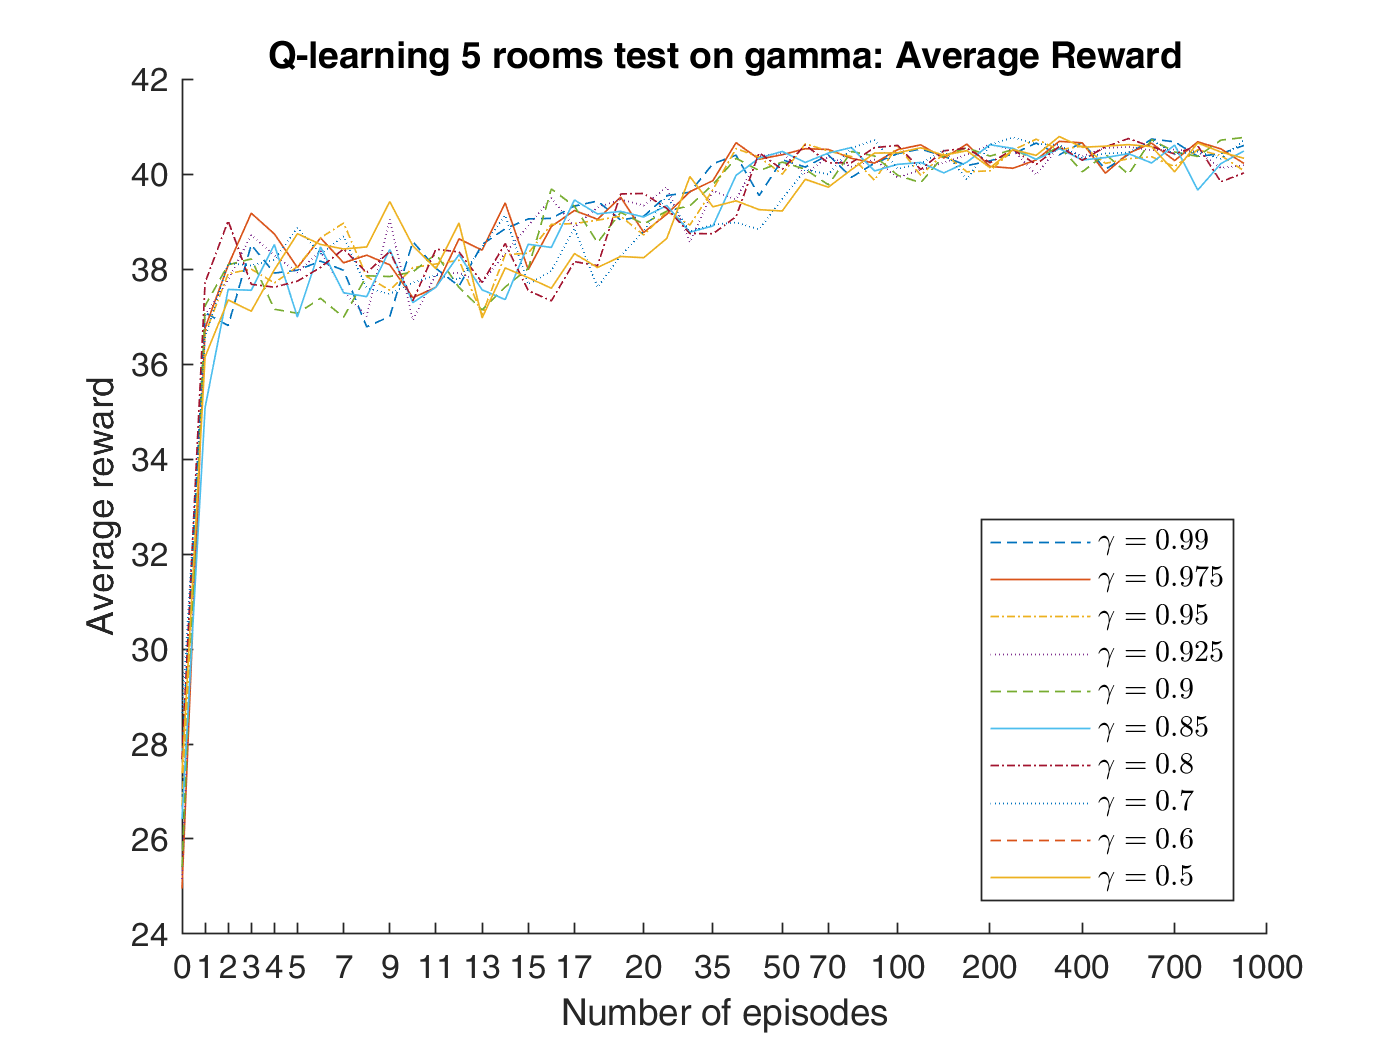
\includegraphics[width=\textwidth]{MatlabPlots/q_learning_5_rooms_test_gamma_average_reward}
		\caption{Plot of how the average reward develops as a function of the number of episodes for each value of $\epsilon$}
		\label{fig:q-learn_gamma_reward}
	\end{subfigure}
	\hfill
	\begin{subfigure}[b]{0.49\textwidth}
		\centering
		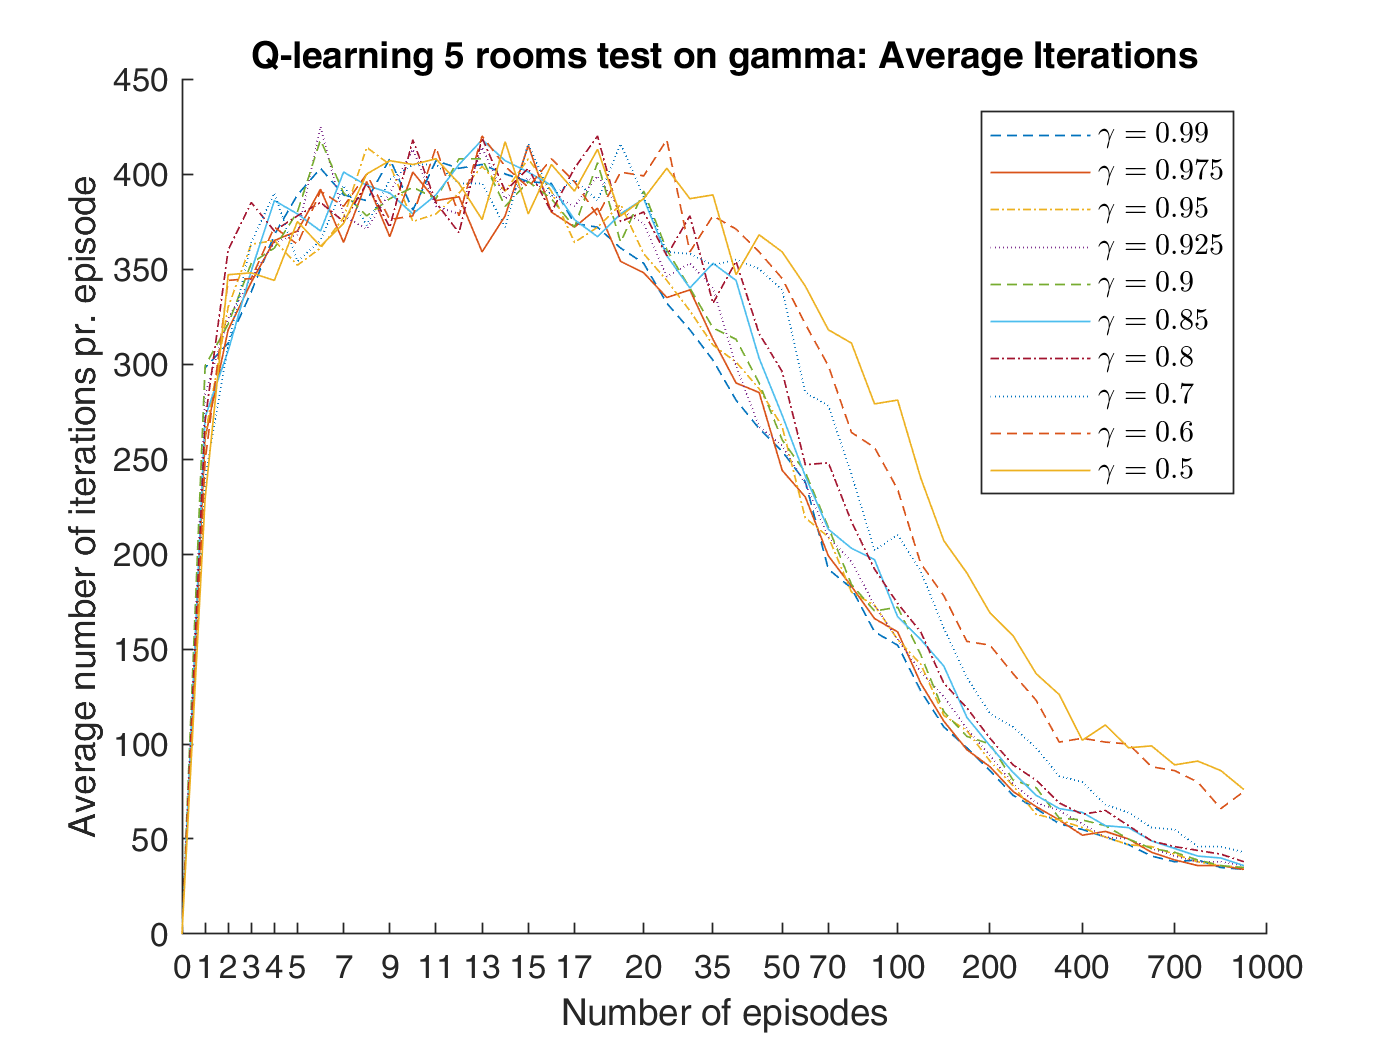
\includegraphics[width=\textwidth]{MatlabPlots/q_learning_5_rooms_test_gamma_average_iterations}
		\caption{Plot of how the average number of episodes develops as a function of the number of episodes for each value of $\alpha$}
		\label{fig:q-learn_gamma_iterations}
	\end{subfigure}
	\caption{Plots of both the average reward and average number of iterations pr. episode for each value of $\gamma$}
	\label{fig:q-learn_gamma}
\end{figure}
A value of 0.99 have been chosen as the best compromise between a high average reward and a low average number of iterations per episode.

\subsubsection*{Conclusion}
It can be concluded that the higher the value of $\gamma$ the higher the average reward will be for a given number of episodes.\\
It can as well be concluded that the higher the value of $\gamma$ the lower the number of iterations per episode will be.\\ 
The value of 0.99 was chosen as the best compromise.


\end{document}